%//==============================--@--==============================//%
\subsection[3.2 Multiplexação e Desmultiplexaçãol]{\hspace*{0.075 em}\raisebox{0.2 em}{$\pmb{\drsh}$} Multiplexação e Desmultiplexação}
\label{subsec:multiplex-demultiplex}


\begin{theo}[\underline{Multiplexing and demultiplexing}]{teo/def:Multi-Demu}\label{def:Multi-Demu}
    ``At the destination host, the transport layer receives segments from the network layer just below. The transport layer has the responsibility of delivering the data in these segments to the appropriate application process (socket) running in the host. (...) \textbf{This job of delivering the data in a transport-layer segment to the correct socket is called} \textbf{demultiplexing}. \textbf{The job of gathering data chunks at the source host from different sockets, encapsulating each data chunk with header information to create segments}, and passing the segments to the network layer \textbf{is called multiplexing}" 
\end{theo}

\noindent A multiplexação e a desmultiplexação está dependente da identificação única inerente às \textit{sockets} e requer que cada segmento da camada de transporte possua um \textbf{source port number} field e um \textbf{destination port number} field (\textit{vide} \hyperref[appendixB]{Appendix C: Reserved Ports}).

\begin{figure}[H]
    \centering
    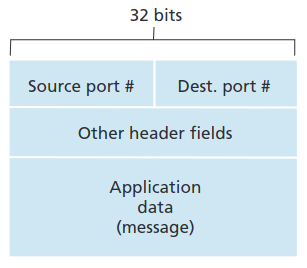
\includegraphics[width = 0.45\linewidth]{img/3/segment.png}
    \caption{Estrutura de um segmento da camada de transporte.\protect\cite{Kurose2017}}
    \label{fig:segment}
\end{figure}

\noindent Os restantes \textit{header fields} estão dependentes do tipo de protocolo em uso, nomeadamente, \textbf{UDP} e \textbf{TCP}.

%//==============================--@--==============================//%